\chapter{Weakly and strongly Hausdorff}

In this chapter we will consider two point-free analogies of the $T_2$ axiom:
a~separation not quite easy to imitate in frames.

\section{The $T_2$ axiom}

\begin{framed}
  \begin{df}[$T_2$]
    A topological space $(X, \tau)$ is called \emph{Hausdorff\/} (also equally
    a~\emph{$T_2$-space\/}) if
    \begin{center} \it
      for any $x \ne y$ from~$X$ there are disjoint $U$ and $V$ with $U\owns x$
      and $V\owns y$.
    \end{center}
  \end{df}
\end{framed}

\begin{figure}[h]
  \centering
  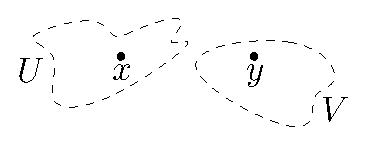
\includegraphics[height=13mm]{../img/t2.eps}
  \caption{$T_2$ property}
\end{figure}

\begin{rem} \label{T2->T1}
  Trivially, every $T_2$-space is $T_1$.
\end{rem}

\section{The Dowker-Strauss approach}

In 1972 Dowker and Strauss \cite{ds72} introduced the following condition:

\begin{framed}
  \begin{df}
    A locale $L$ satisfies the $S_2'$ axiom if
    \[
      (S_2') \qquad
      a, b \ne 1 \text{ and } a \vee b = 1 \quad \Rightarrow \quad \exists
      u\not\leq a, v\not\leq b, \quad u \wedge v = 0.
    \]
  \end{df}
\end{framed}

Its relationship to the Hausdorff property is seen from following
\begin{thm} \label{thm:T2=S2'+Sfit}
  For the $\Omega(X)$ of any topological space $X$ we have
  \[
    (T_2) \; \equiv \; (S_2') \& (\text{Sfit}).
  \]
\end{thm}

\begin{lem} \label{Haus->S2'}
  The $\Omega(X)$ of a~Hausdorff $X$ satisfies $S_2'$.
\end{lem}
\begin{proof}
  Open sets $A, B \ne X$ with $A \cup B = X$ contain some $x\in X\setminus A =
  B\setminus A$ and some $y\in X\setminus B = A\setminus B$.
  Particularly, we observe $x \ne y$ and, on top of that, receive the disjoint
  $U$ and $V$ from $(T_2)$.
  Also, $U\not\subseteq A$ (because of $x$) and $V\not\subseteq B$ (because of
  $y$).
\end{proof}

\begin{lem} \label{lem:S2'+Sfit->T1}
  $(S_2') \& (\text{Sfit}) \, \Rightarrow \, (T_1)$.
\end{lem}
\begin{proof}
  Using Fact~\ref{T1Char} on page~\pageref{T1Char}, we will show that $\{ x \}
  = \overline{\{ x \}}$.

  Assume, for the sake of contradiction, that there is $z\in \overline{\{ x \}}
  \setminus \{ x \}$.
  Since we still suppose $(T_0)$, we have $x\not\in \overline{\{ z \}}$.
  Recall Proposition~\ref{Sfit-char} on~page~\pageref{Sfit-char} and consider
  $y\in \overline{\{x\}}$ with $\overline{\{y\}} \subseteq X\setminus
  \overline{\{ z \}}$, i. e., $\overline{\{ y \}} \cap \overline{\{ z \}} =
  \none$.

  For open $A := X \setminus \overline{\{ y \}}$ and $B := X \setminus
  \overline{\{ z \}}$ we have $A \cup B = X$, and hence, also the $U, V$
  from~$(S_2')$.
  Thus, there must be $y'\in \overline{\{ y \}} \cap U$, and consequently,
  $y\in U$ (else $y'\in U\not\owns y$ would lead to $y'\not\in \overline{\{ y
  \}}$).
  Likewise, $z\in V$.
  However, $U$ and $V$ cannot be disjoint:
  as $y\in \overline{\{ x \}}$ resp. $z\in \overline{\{ x \}}$ implies $x\in U$
  resp. $x\in V$.
\end{proof}

\begin{lem} \label{lem:S2'+T1->T2}
  $(S_2') \& (T_1) \, \Rightarrow \, (T_2)$.
\end{lem}
\begin{proof}
  For open $A := X\setminus \{ x \}$ and $B := X\setminus \{ y \}$ take the
  disjoint $U, V\in \Omega(X)$ from $(S_2')$.
  Thus, $U\not\subseteq A$ resp. $V\not\subseteq B$ translates to $U\owns x$
  resp. $V\owns y$.
\end{proof}

\begin{proof}[Proof of~{\bf\ref{thm:T2=S2'+Sfit}}]
  ~

  $\Rightarrow$:
  By~\ref{T2->T1} and \ref{T1->Sfit} (on page~\pageref{T1->Sfit}), we get the
  subfitness, and using~\ref{Haus->S2'}, also the axiom $(S_2')$.

  $\Leftarrow$:
  Apply lemmata \ref{lem:S2'+Sfit->T1} and \ref{lem:S2'+T1->T2}.
\end{proof}

The $(S_2')$ axiom is often replaced by a~somewhat stronger condition:

\begin{framed}
  \begin{df}[DS-Haus]
    A locale $L$ is said to be \emph{weakly Hausdorff\/} (also
    \emph{DS-Hausdorff} as in \emph{Dowker-Straus-Hausdorff}) if
    \[
      a \vee b \not\in \left\{a, b\right\} \qquad \Rightarrow \qquad \exists
      u\not\leq a, v\not\leq b, \quad u \wedge v = 0.
    \]
  \end{df}
\end{framed}

\begin{prop} \label{prop:DS-Haus->S2'}
  (DS-Haus) implies $(S_2')$.
\end{prop}
\begin{proof}
  If $a \vee b = 1$ and $a, b \ne 1$ then $a \vee b\not\in \{ a, b \}$.
\end{proof}

\section{Isbell's approach}

Here is a~characterization of~the classical~$T_2$:

\begin{prop}
  A topological space $X$ is Hausdorff space if and only if the~diagonal
  $\Delta = \left\{(x, x) \st x\in X \right\}$ is closed in the product
  $X\times X$.
\end{prop}

\begin{proof}
  $\Rightarrow:$ Any element $(x, y)\not\in \Delta$, that means $x \ne y$, is
  separable from $\Delta$:
  namely, by~the~open $p_1^{-1}[U] \cap p_2^{-1}[V]$ with non-intersecting $U$
  and $V$ from the definition of~$(T_2)$.
  Hence, $(x, y)\not\in \overline{\Delta}$ concludes to $\Delta =
  \overline{\Delta}$, which is closed.

  $\Leftarrow:$ Choose $x \ne y$, in other words, $(x, y)\not\in \Delta$.
  Then $(x, y)$ has an open basic neighbourhood $U_1\times U_2$ disjoint from
  $\Delta$.
  That is, $U_1 \cap U_2 = \none$.
\end{proof}

This was used by Isbell \cite{isbell72} for the point-free counterpart of the
$T_2$ axiom:
Hausdorff locales are defined as those in which the~codiagonal (see
page~\pageref{codiag-in-Frm})
\[
  \nabla\colon L \oplus L \to L
\]
is a closed sublocale (see page~\pageref{df:closed-sloc}).
Since $\nabla(U) \le 0 \, \equiv \, U \subseteq \Delta(0)$, the closure of~the
codiagonal (recall \ref{prop:sloc-closure}) is $\check{d_L} = (U
\mapsto U \vee d_L)$ where
\[
  d_L
  = \bigvee \{ U \st \nabla(U) = 0 \}
  = \bigvee \{ U \st U \subseteq \Delta(0) \}
  = \Delta(0).
\]
Following from Corollary~\ref{cor:closed-sloc}, the condition proposed by
Isbell reduces~to

\begin{framed}
  \begin{df}[I-Haus]
    A locale $L$ is \emph{strongly Hausdorff\/} (or \emph{I-Hausdorff}: short
    for \emph{Isbell-Hausdorff}) if there is a~mapping $\alpha\colon L \to
    \dL$ such that
    \[
      \alpha \nabla = (U \mapsto U \vee d_L).
    \]
  \end{df}
\end{framed}

Note that the isomorphism~$\alpha$ has to be the restriction of~$\Delta$ to $L
\to \dL$.
We~have $\alpha^{-1} \check{d_L} = \nabla$, and hence,
\[
\Delta
= \nabla_*
= (\alpha^{-1} \check{d_L})_*
= (\check{d_L})_* \alpha
= j \alpha
\]
because the embedding $j\colon \dL \embed L \oplus L$ is the right adjoint
to~$\check{d_L}$ (see \ref{lem:embed-adjoint}).

\begin{lem} \label{lem:IHaus->dL}
  In an~I-Hausdorff locale~$L$ it holds that $\Delta[L] = \dL$.
\end{lem}
\begin{proof}
  As $\alpha$ is the restriction of~$\Delta$ and also an~isomorphism, we get
  $\Delta[L] = \alpha[L] = \dL$.
\end{proof}

\begin{thm} \label{IHaus->DSHaus}
  (I-Haus) implies (DS-Haus).
\end{thm}

\begin{lem} \label{lem:delta-nabla=id}
  In case of a strongly Hausdorff locale $L$, we have
  \[
    \Delta\nabla(U) = U
  \]
  for any saturated $U \supseteq d_L$.
\end{lem}
\begin{proof}
  By Lemma~\ref{lem:IHaus->dL}, every saturated $U\in \dL = \Delta[L]$ is an
  image $\Delta(a)$ for some $a\in L$.
  Let us write $\delta(U)$ for this $a$.
  In other words, $\Delta\delta(U) = U$.

  The frame codiagonal is an epimorphism and hence---as~we have $\nabla \Delta
  \nabla = \nabla$ by Fact~\ref{lrl=l} on page~\pageref{lrl=l}---we also get
  $\nabla \Delta = id$.

  Joining these two observations:
  \[
    \nabla (U) = \nabla (\Delta\delta (U)) = (\nabla \Delta)\delta (U) =
    \delta(U),
  \]
  which produces the desired $U = \Delta \delta (U) = \Delta \nabla (U)$.
\end{proof}

\begin{prop} \label{meets-in-satur}
  A~locale~$L$ is I-Hausdorff iff one has the~implication
  \begin{equation} \label{eq:meets-in-satur}
    \left( a \wedge b, a \wedge b \right) \in U
    \; \Rightarrow \;
    \left( a, b \right) \in U
  \end{equation}
  for all saturated $U \supseteq d_L$.
\end{prop}
\begin{proof}
  $\Rightarrow$:
  Whenever $(a \wedge b, a \wedge b)\in U$, we see from the formula for
  $\nabla$ that
  \[
    a \wedge b \leq \bigvee \left\{ x \st (x, x) \in U \right\} = \nabla(U).
  \]
  Having in mind the formula for $\Delta$, immediately $(a, b) \in \Delta(
  \nabla(U) ) = U$
  (the final equality by Lemma~\ref{lem:delta-nabla=id}).

  $\Leftarrow$:
  Let the condition hold and~let $a_i\in L$ for $i\in J$. 
  Since for any~saturated down-set~$U \supseteq d_L$ we have $(a_i, a_i) \in U
  \Rightarrow (a_i \wedge a_j, a_i \wedge a_j) \in U$, we also obtain
  the~implication
  \begin{equation} \label{eq:IHaus-impl}
    (a_i, a_i) \in U \Longrightarrow \{ (a_i, a_j) \st j\in J \} \subseteq U
    %\tag{\arabic{chapter}.\thesection}
  \end{equation}

  We will prove that $\alpha := (a \mapsto (a \oplus a) \vee d_L)$ satisfies
  the definition.
  Using
  \[
    \bigvee_{i\in J} a_i \oplus \bigvee_{j\in J} a_j
    = \iota_1 \left( \bigvee_{i\in J} a_i \right) \wedge \iota_2 \left(
    \bigvee_{j\in J} a_j \right)
    = \bigvee_{i, j\in J} \left( \iota_1(a_i) \wedge \iota_2(a_j) \right)
    = \bigvee_{i, j\in J} \left( a_i \oplus a_j \right)
  \]
  (the latter equality by double application of frame distributivity), we see
  that $\alpha$~preserves suprema:
  \begin{align*}
    \alpha \left( \bigvee_{i\in J} a_i \right)
    &= \left(\bigvee_{i, j\in J} \left( a_i \oplus a_j \right)\right) \vee d_L
    = \bigvee_{i\in J} \left(\left( a_i \oplus a_i \right) \vee d_L \right)
    = \bigvee_{i\in J} \alpha \left( a_i \right)
  \end{align*}
  (by~\eqref{eq:IHaus-impl} the second and the third expressions have identical
  upper bounds).
  Thus, both $\alpha$ and $\nabla$ preserve joins and~so does $\alpha \nabla$. 

  Furthermore, we have
  \[
    \alpha \nabla (a \oplus b)
    = \alpha (a \wedge b)
    = ((a \wedge b) \oplus (a \wedge b)) \vee d_L
    = (a \oplus b) \vee d_L,
  \]
  the last equality stipulated by assumed implication
  \eqref{eq:meets-in-satur}.

  In~conclusion,
  \begin{flalign*}
    \alpha \nabla (U)
    &= \alpha \nabla \left(\bigvee \{a \oplus b \st (a, b)\in U\}\right)
    = \bigvee \{\alpha \nabla \left(a \oplus b \right) \st (a, b)\in U\} \\
    &= \bigvee \{a \oplus b \vee d_L \st (a, b)\in U\}
    = \bigvee \{a \oplus b \st (a, b)\in U\} \vee d_L
    = U \vee d_L,
  \end{flalign*}
  as the elements $a \oplus b$ generate $L \oplus L$ (see
  page~\pageref{a+b-gen}).
\end{proof}

\begin{lem} \label{downsets-satur}
  The down-set
  \[
    U = \left\downarrow(a, a \wedge b)\right. \cup \left\downarrow(a \wedge b,
        b)\right. \cup \n
  \]
  is saturated in $L \times L$ for arbitrary $a, b\in L$.
\end{lem}
\begin{proof}
  Recall the saturatedness on~page~\pageref{df:satur}.
  First of all, let us have $(x_i, y)\in U$ for $i\in J$.

  \underline{Case $y = 0$}:
  obviously, $(\bigvee_{i\in J} x_i, y) = (\bigvee_{i\in J} x_i, 0)\in \n$.

  \underline{Case $y \ne 0$ and $y \leq a \wedge b$}:
  then it must be that $x_i \leq a$ in~any case.
  Thus, $(\bigvee_{i\in J} x_i, y) \in \left\downarrow(a, a \wedge b).\right.$

  \underline{Case $y \ne 0$ and $y \not\leq a \wedge b$}:
  we have both $y \leq b$ and $x_i \leq a \wedge b$.
  Hence, again $(\bigvee_{i\in J} x_i, y) \in \left\downarrow(a \wedge b,
  b)\right. \subseteq U$.

  The $(x, \bigvee_{i\in J} y_i)$ by symmetry.
\end{proof}

\phantomsection
\label{sec:overline S2}
Now we can prove the theorem.
In fact, we are going to imply a~stronger version of the (DS-Haus):
\[
  a \vee b \not\in \left\{a, b\right\} \qquad \Rightarrow \qquad \exists
  u\not\leq b, v\not\leq a: \quad u \wedge v = 0, \quad \boxed{\left(u,
  v\right) \leq \left(a, b\right)}
\]

\begin{proof}[Proof of~{\bf \ref{IHaus->DSHaus}}]
  For a contradiction: let there be an I-Hausdorff $L$, which is not weakly
  Hausdorff.
  That means, we have $a, b$ with $a \not\leq b, \, b \not\leq a$ and such that
  \[
    u \wedge v = 0 \quad \& \quad \left(u, v\right) \leq \left(a, b\right)
    \qquad \Longrightarrow \qquad
    u \leq b \; \textrm{ or } \; v \leq a.
  \]
  Especially, for the down-set $U$ taken from~\ref{downsets-satur} we have
  \begin{equation} \label{eq:dl-aoplusb}
    d_L \cap (a \oplus b) \subseteq U.
  \end{equation}

  Following from~\ref{meets-in-satur}, the saturated $(\left(a \wedge b\right)
  \oplus \left(a \wedge b\right)) \vee d_L \supseteq d_L$ contains $(a, b)$
  as it trivially contains $\left( a \wedge b, a \wedge b \right)$.
  Hence,
  \begin{align*}
    (a, b) &\in (a \oplus b) \; \cap \; (((a \wedge b) \oplus (a \wedge b))
            \vee d_L) \\
           &= ((a \wedge b) \oplus (a \wedge b)) \; \vee \; ((a \oplus b) \cap
               d_L) \\
           &\subseteq ((a \wedge b) \oplus (a \wedge b)) \; \vee \; U \\
           &= U.
  \end{align*}
  The first equality using~distributivity and the fact that $(a \wedge b)
  \oplus (a \wedge b) \subseteq a \oplus b$;
  the inclusion by~(\ref{eq:dl-aoplusb});
  the final equality from $(a \wedge b) \oplus (a \wedge b) \subseteq U$.

  This leads to the contradiction:
  $(a, b)\not\in \n$ since neither $a$ nor $b$ may equal $0$ (by $a \not\leq b,
  \, b \not\leq a$).
  Thus, the only options available are either $a \leq a \wedge b$ or $b \leq a
  \wedge b$.
  However, those stipulate $a \leq b$ or $b \leq a$ respectively,
  a~contradiction. 
\end{proof}
